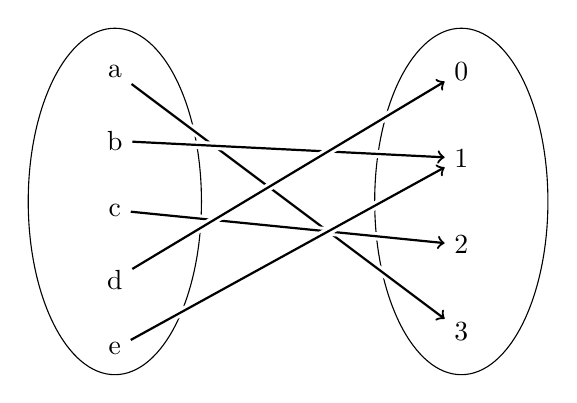
\begin{tikzpicture}[scale=1.1]
% sets
    \draw (0,0) ellipse (1cm and 2cm);
    \draw (4,0) ellipse (1cm and 2cm);
    \foreach \y/\v in {0/a,1/b,2/c,3/d,4/e}{
        \node (\v) at (0,1.5-4/5*\y) {\v};
    }
    \foreach \y/\v in {0,1,2,3}{
        \node (\y) at (4,1.5-\y) {\y};
    }
% function
    \foreach \y/\v in {3/a,1/b,2/c,0/d,1/e}{
        \draw[line width=3pt, white] (\v) -- (\y);            
        \draw[->,thick] (\v) -- (\y);
    }
\end{tikzpicture}        
